% Provenance (never printed): old terminale S material on the early Earth (the
% primitive atmosphere and its outgassing, the first traces of life, the rise of
% oxygen read in the rocks: banded iron formations, red beds) and the faint young
% Sun. Owner (Sync 0/1): outgassing and primitive atmosphere, faint young Sun
% problem, stromatolite, Great Oxidation Event, banded iron formation, red beds.
% Recalled: age of the Earth (g12.07), zircons (g12.01), equilibrium temperature
% (g10.02), photosynthesis and cyanobacteria (biology), air composition, greenhouse
% gases as molecules and redox (chemistry). Figures: figdata/grade-12/early_earth.py.
\chapter{De jonge Aarde en haar atmosfeer}\label{ch:g12:early-earth}

In de Hamersley Ranges, in het noordwesten van Australië, zijn de wanden van Dales Gorge
gestreept als een laagjestaart: dunne banden van rood, grijs en zwart gesteente. Ze
vormen een \omterm{def:g12:early-earth:bif}{gebande ijzerformatie}, afgezet op een zeebodem meer dan 2.5 miljard
jaar geleden.
Het ijzer erin roestte in die zee, en om te roesten had het zuurstof nodig. Dit
hoofdstuk vraagt hoe de jonge Aarde en haar lucht eruitzagen, en hoe de gesteenten
het moment vastleggen waarop zuurstof verscheen.
% ledger: dbca:karijini, earle:bif, photo:g12-dales-gorge

\begin{omfigure}
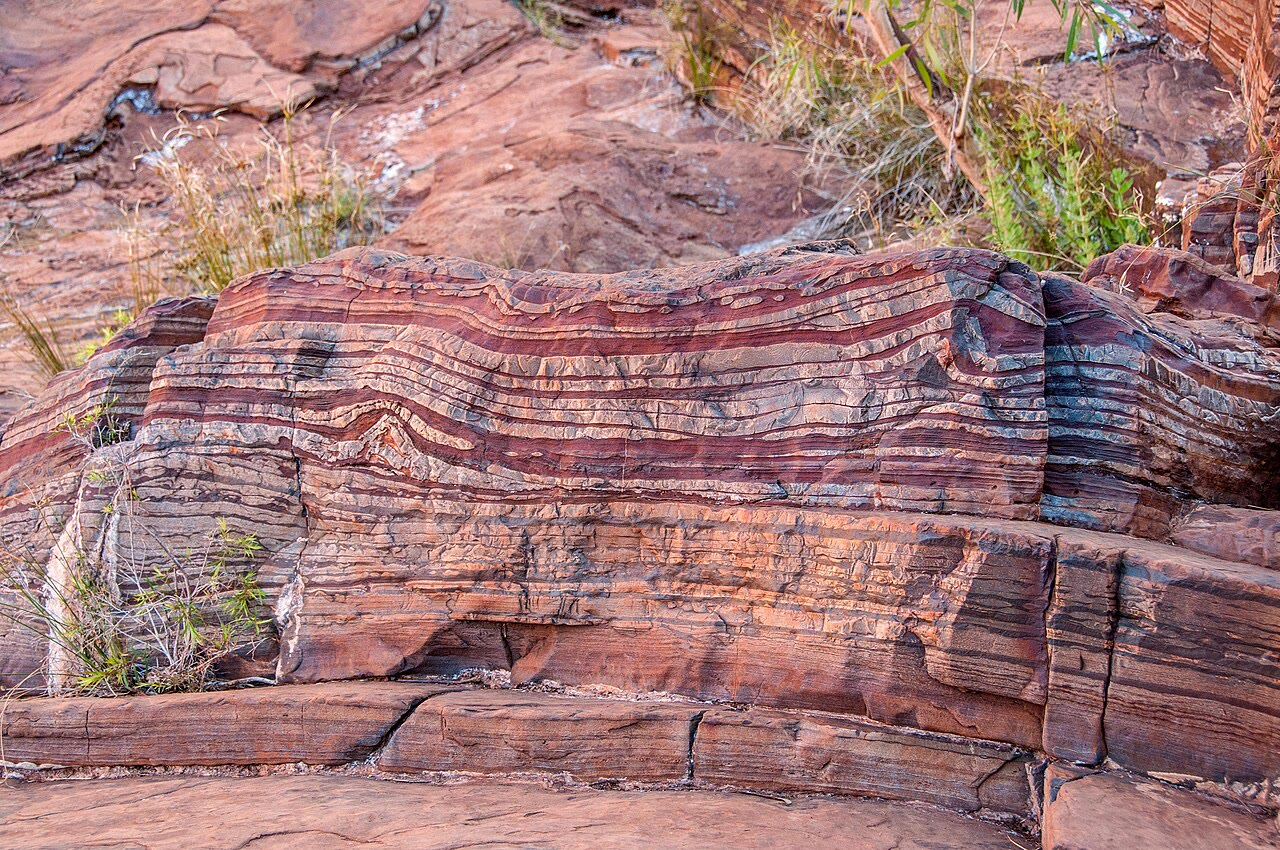
\includegraphics[width=0.72\linewidth]{images/book2/g12-dales-gorge-bif.jpg}

{\small \omterm{def:g12:early-earth:bif}{Gebande ijzerformatie} bij Fortescue Falls, Dales Gorge, Karijini
National Park, West-Australië. Foto Graeme Churchard, CC~BY~2.0
(Wikimedia Commons).}
\end{omfigure}

\begin{recall}
De Aarde is 4.54 miljard jaar oud (\cref{ch:g12:age-of-the-earth}), en
zirkoonkorrels tonen dat er 4.4 miljard jaar geleden een korst bestond
(\cref{ch:g12:continental-crust}). De \omterm{def:g10:habitable-planet:equilibrium-temperature}{evenwichtstemperatuur} van een planeet,
$T_{\mathrm{eq}} = \left(S(1-A)/(4\sigma)\right)^{1/4}$, is ongeveer \qty{255}{K}
voor de Aarde van vandaag (\cref{ch:g10:habitable-planet}). Droge lucht bestaat vandaag voor
\qty{78}{\percent} uit stikstof en voor \qty{21}{\percent} uit zuurstof, en koolstofdioxide en
methaan zijn broeikasgassen; een element dat zuurstof opneemt, wordt geoxideerd (de
scheikundeboeken). Planten, algen en cyanobacteriën maken hun voedsel door
fotosynthese, waarbij zuurstof vrijkomt (de biologieboeken).
\end{recall}
% ledger: usgs:age-earth (Book 1 row), wilde01:zircon, earth:TSI, earth:albedo, air:N2, air:O2

\section{De jonge Aarde}

De Aarde groeide door het samenklonteren van kleinere hemellichamen. Ongeveer 60 miljoen jaar
nadat het zonnestelsel begon te ontstaan, trof een hemellichaam, misschien zo groot als Mars,
haar, en het materiaal dat de ruimte in werd geslingerd, vormde de Maan. De jonge Aarde was
heet en nog deels gesmolten. Ze koelde af, en ongeveer 4.4 miljard jaar geleden
had ze al een korst en een oceaan: zirkoonkorrels van die ouderdom dragen het scheikundige spoor
van vloeibaar water.
% ledger: nasa:moon-formation, wilde01:zircon

\section{De oeratmosfeer}

\begin{definition}[Ontgassing; oeratmosfeer]\label{def:g12:early-earth:primitive-atmosphere}
\emph{Ontgassing}\index{ontgassing} is het vrijkomen, door vulkanen en door
de grond heen, van de gassen die in magma zijn opgelost. De \emph{oeratmosfeer}\index{oeratmosfeer} is de atmosfeer van de Aarde voordat
levende wezens haar veranderden: grotendeels door ontgassing opgebouwd, bevatte ze stikstof,
koolstofdioxide en waterdamp, meer koolstofdioxide dan vandaag, en bijna
geen vrije zuurstof.
\end{definition}
% ledger: usgs:volcanic-gases (Book 1 row), holland06:stages (stage 1 anoxic), feulner12:fys (more carbon dioxide)

Vulkanen tonen nog altijd hoe zo'n atmosfeer ontstaat: wanneer magma opstijgt en de
druk daalt, ontsnappen zijn opgeloste gassen, waarvan waterdamp verreweg het overvloedigst is,
gevolgd door koolstofdioxide. Stikstof en koolstofdioxide, de gassen
die de oerlucht beheersten, zijn vandaag nog de voornaamste stikstof- en
koolstofhoudende gassen van vulkanen. De waterdamp condenseerde tot de
oceaan. Zuurstof bedroeg minder dan \qty{0.001}{\percent} van zijn niveau in de lucht van
vandaag.
% ledger: usgs:volcanic-gases (Book 1 row), pk02:anoxic

De jonge Zon scheen minder fel dan vandaag. Terwijl ze in haar kern waterstof in
helium omzet, trekt de kern samen en warmt op, en het vermogen van de Zon
neemt langzaam toe.

\begin{proposition}[De lichtkracht van de jonge Zon]\label{prop:g12:early-earth:luminosity}
Noem $t_\odot$ de huidige ouderdom van de Zon en $L_\odot$ haar huidige
lichtkracht; haar lichtkracht toen ze $t$ jaar oud was, was dan
\[
  L(t) = \frac{L_\odot}{1 + \frac{2}{5}\left(1 - t/t_\odot\right)} .
\]
\end{proposition}
% ledger: gough81:luminosity, connelly12:cai

Deze benadering van de berekende modellen van de Zon wordt hier aangenomen. Bij de
geboorte van de Zon, $t = 0$, geeft ze $L = L_\odot/1.4 \approx 0.71\,L_\odot$:
de jonge Zon was ongeveer \qty{30}{\percent} zwakker.

\begin{example}[De Aarde vier miljard jaar geleden]\label{ex:g12:early-earth:young-sun}
Neem $t_\odot = 4.567$ miljard jaar. Vier miljard jaar geleden was de Zon
0.567 miljard jaar oud, dus $1 - t/t_\odot = 4/4.567 \approx 0.876$ en
$L \approx L_\odot/1.350 \approx 0.741\,L_\odot$. Het zonlicht dat de
Aarde bereikte, was $0.741 \times 1361 \approx \qty{1008}{W/m^2}$. Bij het
\omterm{def:g10:earth-energy-budget:albedo}{albedo} van vandaag schaalt de \omterm{def:g10:habitable-planet:equilibrium-temperature}{evenwichtstemperatuur} met de vierdemachtswortel van het
zonlicht: $255 \times 0.741^{1/4} \approx 255 \times 0.928 \approx
\qty{237}{K}$, ongeveer \qty{-36}{\celsius}.
\end{example}
% values: L_4Ga 0.7406, S_4Ga 1007.9, Teq_today 255.1, Teq_4Ga 236.7 (early_earth.py)

\begin{omfigure}
\begin{tikzpicture}
\begin{axis}[omrecord, scale only axis, width=0.66\linewidth, height=4.6cm,
  xmin=0, xmax=4.6, ymin=225, ymax=295, x dir=reverse, axis y line*=left,
  xlabel={tijd vóór heden (miljard jaar)}, ylabel={temperatuur (K)},
  xtick={0,0.5,...,4.5}, x tick label style={/pgf/number format/.cd, fixed, precision=1}]
% computed in figdata/grade-12/early_earth.py; ledger: gough81:luminosity, earth:TSI, earth:albedo, earth:Tsurf
\addplot[omDef, line width=1.2pt] table[x=t_Ga, y=Teq] {figdata/out/grade-12-early_earth-sun.dat};
\addplot[omThm, densely dashed, domain=0:4.6, samples=2] {273.15};
\addplot[black!60, densely dotted, domain=0:4.6, samples=2] {288};
\coordinate (teq) at (axis cs:2.6,239);
\coordinate (frz) at (axis cs:2.3,274);
\coordinate (sfc) at (axis cs:2.3,289);
\end{axis}
\begin{axis}[omrecord, scale only axis, width=0.66\linewidth, height=4.6cm,
  xmin=0, xmax=4.6, ymin=0.65, ymax=1.05, x dir=reverse, axis y line*=right, axis x line=none,
  ylabel={lichtkracht van de Zon ($L_\odot$)}, ymajorgrids=false, xmajorgrids=false,
  y tick label style={/pgf/number format/.cd, fixed, fixed zerofill, precision=2}]
\addplot[omProp, line width=0.9pt, densely dashdotted] table[x=t_Ga, y=L] {figdata/out/grade-12-early_earth-sun.dat};
\coordinate (lum) at (axis cs:1.7,0.86);
\end{axis}
\node[font=\scriptsize, text=omDef, anchor=north] at (teq) {evenwichtstemperatuur};
\node[font=\scriptsize, text=omThm, anchor=south] at (frz) {water bevriest, \qty{273}{K}};
\node[font=\scriptsize, text=black!70, anchor=south] at (sfc) {gemiddeld oppervlak vandaag, \qty{288}{K}};
\node[font=\scriptsize, text=omProp, anchor=north west] at (lum) {lichtkracht (rechterschaal)};
\end{tikzpicture}

{\small De zwakke jonge Zon: haar lichtkracht (rechterschaal) en de
\omterm{def:g10:habitable-planet:equilibrium-temperature}{evenwichtstemperatuur} van de Aarde bij het \omterm{def:g10:earth-energy-budget:albedo}{albedo} van vandaag (linkerschaal), terug tot de geboorte
van de Zon. Berekend uit Gough (1981) met het zonlicht en het \omterm{def:g10:earth-energy-budget:albedo}{albedo} van vandaag.}
\end{omfigure}

\begin{definition}[Probleem van de zwakke jonge Zon]\label{def:g12:early-earth:faint-young-sun}
Het \emph{probleem van de zwakke jonge Zon}\index{zwakke jonge Zon, probleem van de} is de
tegenspraak tussen de zwakkere Zon van de eerste miljarden jaren van de Aarde,
waaronder de Aarde met de atmosfeer van vandaag zou zijn bevroren, en de
gesteenten, die tonen dat er vloeibaar water was.
\end{definition}
% ledger: feulner12:fys

Het probleem werd in 1972 breed bekend door Carl Sagan en George Mullen,
die een sterker broeikaseffect als antwoord voorstelden. De meeste antwoorden
die sindsdien zijn onderzocht, doen een beroep op meer broeikasgassen in de \omterm{def:g12:early-earth:primitive-atmosphere}{oeratmosfeer}:
veel meer koolstofdioxide dan vandaag, methaan gemaakt door vroege microben, of
beide. In één klassieke berekening houdt ongeveer een tiende bar koolstofdioxide,
met een beetje methaan, de jonge Aarde even warm als vandaag; zonder het
methaan is ongeveer drie keer meer nodig. Het probleem wordt nog niet als
opgelost beschouwd.
% ledger: feulner12:fys

\section{Leven en zuurstof}

De fossiele overlevering van \omterm{def:g12:early-earth:stromatolite}{stromatolieten} bestrijkt bijna \num{3500} miljoen jaar:
ze behoren tot de oudste sporen van leven.

\begin{definition}[Stromatoliet]\label{def:g12:early-earth:stromatolite}
Een \emph{stromatoliet}\index{stromatoliet} is een gelaagde heuvel die in
ondiep water wordt opgebouwd door een mat van microben, vooral cyanobacteriën, die
sedimentkorrels vangen en binden en carbonaat laten groeien, laag na laag.
\end{definition}
% ledger: noffke13:stromatolites

Fossiele \omterm{def:g12:early-earth:stromatolite}{stromatolieten} van \num{3430} miljoen jaar oud worden gevonden in de Strelley
Pool Chert van de Pilbara, in West-Australië. Levende groeien vandaag in
het zeer zoute water van Hamelin Pool in Shark Bay, dat twee keer zo zout is als gewoon
zeewater, waar ze het bekendste moderne voorbeeld zijn.
% ledger: allwood06:spc, noffke13:stromatolites, dbca:hamelin

\begin{omfigure}
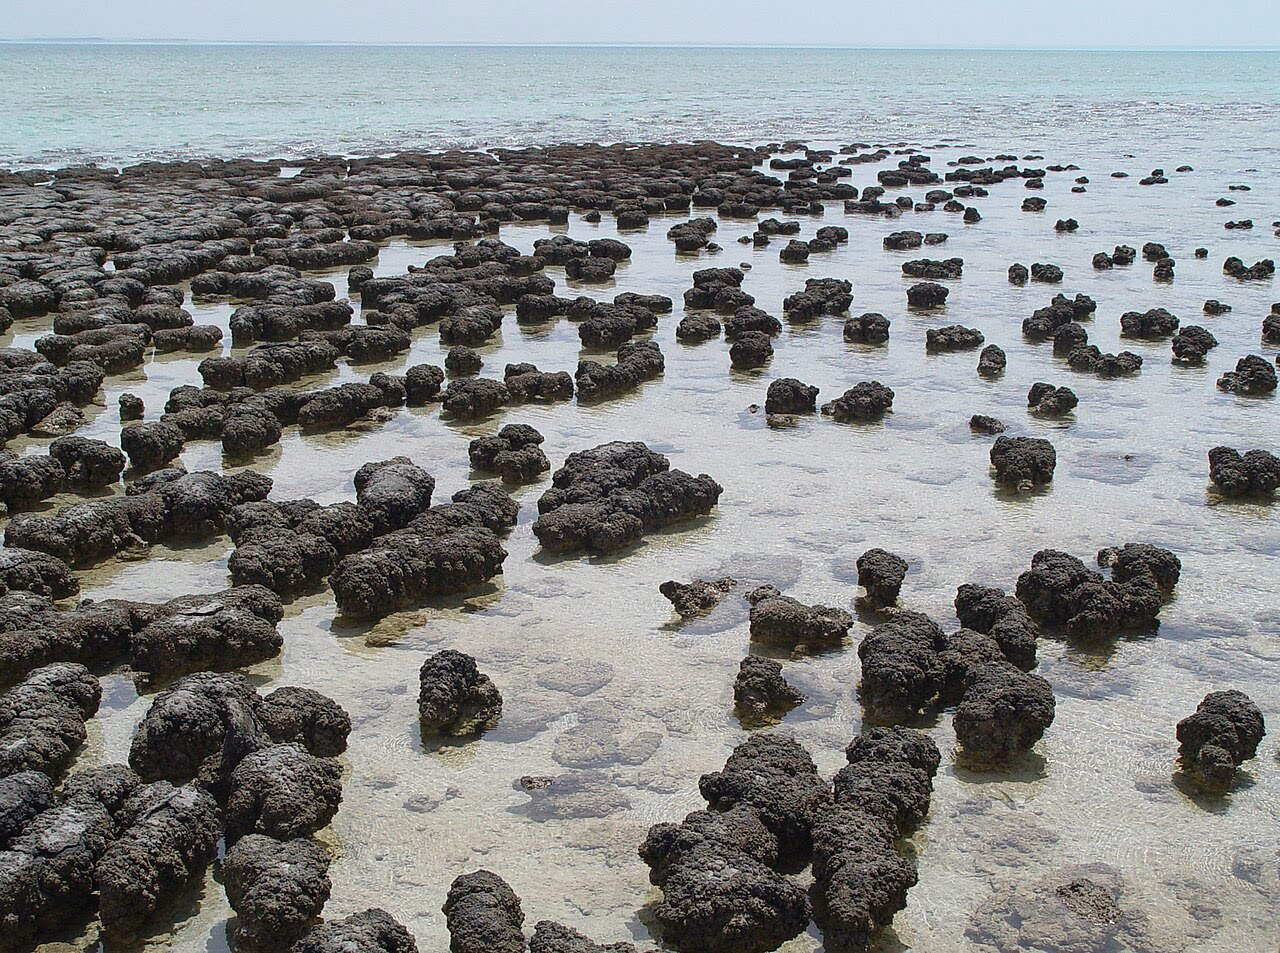
\includegraphics[width=0.6\linewidth]{images/book2/g12-shark-bay-stromatolites.jpg}

{\small Levende \omterm{def:g12:early-earth:stromatolite}{stromatolieten} in Hamelin Pool, Shark Bay, West-Australië.
Foto Paul Harrison, CC~BY-SA~3.0 (Wikimedia Commons).}
\end{omfigure}
% ledger: photo:g12-shark-bay

De cyanobacteriën brachten iets nieuws: fotosynthese waarbij
zuurstof vrijkomt. Maar lange tijd bleef de zuurstof die ze maakten niet in de lucht. Ze
werd even snel verbruikt als ze werd gemaakt: door het ijzer dat in de zee was opgelost, door
zwavel en door methaan.

\section{De opkomst van zuurstof}

Vóór de zuurstof kon ijzer opgelost in zeewater reizen, als het ion
\ce{Fe^2+}. Zuurstof zet het om in ijzer(III), dat niet oplost: het zakt
naar de bodem als een roestkleurig sediment.

\begin{proposition}[IJzer neemt zuurstof op]\label{prop:g12:early-earth:iron}
Opgelost ijzer(II) wordt in water door zuurstof geoxideerd tot ijzer(III)hydroxide,
dat neerslaat:
\[
  \ce{4Fe^2+ + O2 + 10H2O -> 4Fe(OH)3 + 8H+} .
\]
Elke zuurstofmolecule verwijdert vier ionen opgelost ijzer; zolang er
opgelost ijzer overblijft, wordt de gemaakte zuurstof verbruikt.
\end{proposition}
% ledger: earle:bif (ferrous iron oxidised to insoluble ferric iron)

\begin{proof}
Controleer de balans. IJzer: 4 aan elke kant. Zuurstof: $2 + 10 = 12$ links,
$4 \times 3 = 12$ rechts. Waterstof: $20$ links, $4 \times 3 + 8 =
20$ rechts. Lading: $4 \times (+2) = +8$ links, $8 \times (+1) =
+8$ rechts.
\end{proof}

\begin{definition}[Gebande ijzerformatie]\label{def:g12:early-earth:bif}
Een \emph{gebande ijzerformatie}\index{gebande ijzerformatie} is een
sedimentair gesteente van dunne, afwisselende lagen van ijzeroxiden, zoals
hematiet, en van chert, een fijnkorrelig siliciumdioxidegesteente dat arm is aan ijzer. Bijna alle zijn
ouder dan 1.8 miljard jaar.
\end{definition}
% ledger: earle:bif, holland06:stages

\omterm{def:g12:early-earth:bif}{Gebande ijzerformaties} hebben twee wateren tegelijk nodig: een \omterm{def:g10:layered-ocean:thermocline}{diepe oceaan} zonder zuurstof,
die opgelost ijzer meevoert, en een ondiepe, door de zon verlichte zee waar cyanobacteriën
zuurstof maken en het ijzer neerslaat. Ze zijn algemeen in gesteenten van 2.4 tot
1.8 miljard jaar oud, en die van de Hamersley Ranges zijn nog ouder.
\omterm{def:g12:early-earth:bif}{Gebande ijzerformaties} zijn een gewoon ijzererts.
% ledger: earle:bif, holland06:stages (Archean BIF, Hamersley), dbca:karijini

\begin{omfigure}
\begin{tikzpicture}[x=1cm, y=1cm, font=\scriptsize]
  % sea and floor
  \fill[omSea] (0,0) rectangle (11,4);
  \fill[omSea!45!white] (0,2.9) rectangle (11,4);
  \draw[omDef!60, line width=0.4pt, densely dashed] (0,2.9) -- (11,2.9);
  \node[anchor=north east, text=omDef] at (10.9,3.95) {verlicht oppervlaktewater};
  \node[anchor=south east, text=omDef, align=right] at (10.9,0.12) {diep water\\zonder zuurstof,\\rijk aan \ce{Fe^2+}};
  % floor with layers
  \foreach \i/\c in {0/red!55!black, 1/black!20, 2/red!55!black, 3/black!20, 4/red!55!black, 5/black!20} {
    \fill[\c] (0,-0.12*\i) rectangle (11,-0.12*\i-0.12);
  }
  \draw[black!60] (0,0) -- (11,0);
  \node[anchor=west] at (11.1,-0.12) {ijzeroxide};
  \node[anchor=west] at (11.1,-0.36) {chert};
  \draw[black!50, line width=0.3pt] (11.05,-0.06) -- (10.6,-0.06);
  \draw[black!50, line width=0.3pt] (11.05,-0.30) -- (10.6,-0.30);
  % upwelling iron
  \foreach \x in {0.5,1.0,1.5} {
    \draw[-{Stealth}, omDef, line width=0.8pt] (\x,0.4) .. controls (\x+0.4,1.5) and (\x+0.6,2.2) .. (\x+0.9,2.85);
  }
  \node[text=omDef, anchor=west] at (2.3,1.3) {\ce{Fe^2+} stijgt op};
  % cyanobacteria and oxygen
  \foreach \x in {3.8,4.4,5.0,5.6,6.2} {\fill[green!45!black] (\x,3.35) circle (0.07);}
  \node[anchor=south, text=green!35!black] at (5.0,3.47) {cyanobacteriën maken \ce{O2}};
  % reaction
  \node[draw=black!40, fill=white, rounded corners=2pt, inner sep=2pt] at (5.4,2.45) {\ce{4Fe^2+ + O2 + 10H2O -> 4Fe(OH)3 + 8H+}};
  % falling rust
  \foreach \x/\y in {4.6/1.9, 5.0/1.5, 5.5/1.8, 5.9/1.2, 4.3/1.1, 5.2/0.7, 6.1/0.6} {\fill[red!60!black] (\x,\y) circle (0.06);}
  \draw[-{Stealth}, red!60!black, line width=0.6pt] (6.6,2.1) -- (6.6,0.25);
  \node[anchor=west, text=red!60!black, align=left] at (6.7,1.75) {ijzer(III) bezinkt\\als een roestlaag};
\end{tikzpicture}

{\small Hoe een \omterm{def:g12:early-earth:bif}{gebande ijzerformatie} ontstaat (schema, niet op schaal): ijzer
dat is opgelost in het diepe water, dat geen zuurstof bevat, stijgt op tot in de verlichte
zee, waar de zuurstof die cyanobacteriën maken het omzet in ijzer(III), dat
bezinkt. Lagen rijk aan ijzer wisselen af met lagen chert.}
\end{omfigure}

Toen begon zuurstof in de lucht te blijven.

\begin{definition}[Grote Oxidatie]\label{def:g12:early-earth:goe}
De \emph{Grote Oxidatie}\index{Grote Oxidatie} is het
tijdvak, van ongeveer \num{2.46} tot ongeveer \num{2.06} miljard jaar geleden, waarin
vrije zuurstof zich voor het eerst ophoopte in de atmosfeer en de ondiepe zeeën van de Aarde,
tot misschien een tiende van zijn huidige niveau.
\end{definition}
% ledger: gumsley17:goe, holland06:stages (0.02-0.04 atm, about a tenth of 0.21)

Het bewijs zit in de gesteenten. Sommige mineralen, waaronder pyriet en uraniniet,
worden door zuurstof vernietigd; toch worden korrels ervan, door rivieren gerold,
gevonden in oude sedimenten, en korrels pyriet ontbreken in de sedimenten die
na de opkomst van zuurstof zijn afgezet. Zwavelisotopen in gesteenten ouder dan ongeveer 2.45 miljard jaar dragen een
kenmerk dat alleen een lucht met minder dan een honderdduizendste van de zuurstof van vandaag
kan achterlaten; 2.09 miljard jaar geleden is het verdwenen. En op het land verschenen
\omterm{def:g12:early-earth:red-beds}{rode lagen}.
% ledger: kasting25:indicators, pk02:anoxic, farquhar00:sulfur

\begin{definition}[Rode lagen]\label{def:g12:early-earth:red-beds}
\emph{Rode lagen}\index{rode lagen} zijn sedimentaire gesteenten --- zandsteen,
siltsteen, schalie --- die rood gekleurd zijn door een laagje ijzer(III)oxide,
hematiet, op hun korrels. Ze ontstaan alleen waar genoeg zuurstof is om
ijzer te oxideren.
\end{definition}
% ledger: kasting25:indicators (redbeds an oxygen indicator)

\begin{omfigure}
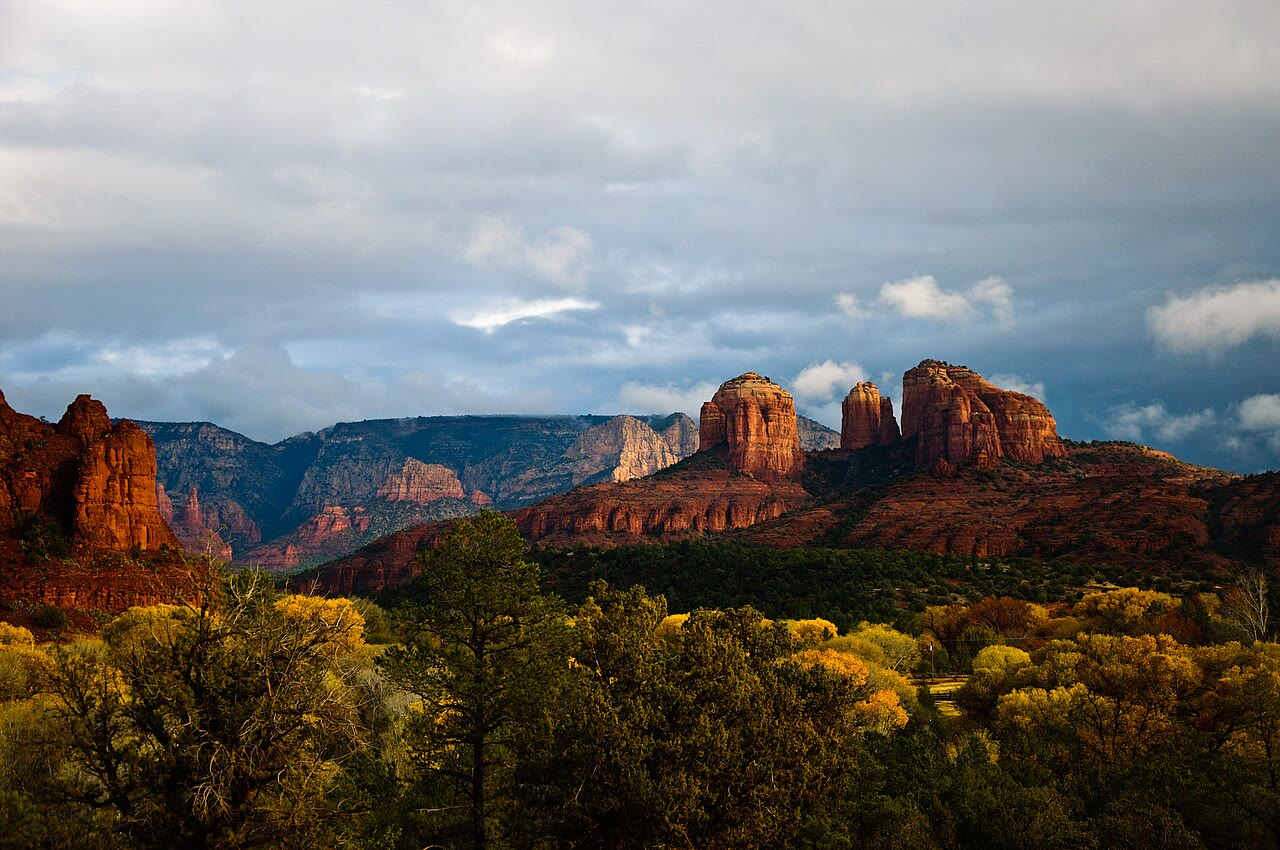
\includegraphics[width=0.66\linewidth]{images/book2/g12-sedona-red-beds.jpg}

{\small \omterm{def:g12:early-earth:red-beds}{Rode lagen}: Cathedral Rock bij Sedona, Arizona, opgebouwd uit rode zandsteen
uit het Perm. Foto Wendy from Pennsylvania, CC~BY-SA~2.0 (Wikimedia
Commons).}
\end{omfigure}
% ledger: photo:g12-sedona, azgs:cathedral (Permian Schnebly Hill Sandstone)

De vorming van \omterm{def:g12:early-earth:bif}{gebande ijzerformaties} hield na 1.8 miljard jaar geleden
in wezen op: toen had ook de \omterm{def:g10:layered-ocean:thermocline}{diepe oceaan} genoeg zuurstof om geen
ijzer meer mee te voeren. In het volgende miljard jaar veranderde de zuurstof weinig; na 0.85 miljard
jaar geleden hoopte ze zich opnieuw op, naar de \qty{21}{\percent} van vandaag.
% ledger: earle:bif, holland06:stages

\begin{method}[Een geologische tijdlijn lezen]\label{met:g12:early-earth:timeline}
\begin{enumerate}
  \item Zoek in welke richting de tijd op de as loopt, en zijn eenheid (miljoenen of
        miljarden jaren vóór heden).
  \item Zoek de eonen op de gekleurde band, en lees hun grenzen af.
  \item Lees voor elke gebeurtenis haar datum af, of het tijdvak waarin ze
        plaatsvond, en zeg welk archief ze dateert (een mineraal, een fossiel, een gesteente).
  \item Bereken tijdsduren door aftrekken, en vergelijk ze met de \omterm{def:g12:age-of-the-earth:age}{ouderdom van
        de Aarde}.
  \item Controleer de volgorde: een gevolg mag niet vóór zijn oorzaak komen.
\end{enumerate}
\end{method}

\begin{omfigure}
\begin{tikzpicture}
\begin{axis}[omrecord, width=0.82\linewidth, height=6.2cm, ymode=log, xmin=0, xmax=4.6, ymin=1e-7, ymax=5,
  x dir=reverse, xlabel={tijd vóór heden (miljard jaar)}, ylabel={zuurstof in de lucht (vandaag $=1$)},
  xtick={0,0.5,...,4.5}, x tick label style={/pgf/number format/.cd, fixed, precision=1},
  ytick={1e-6,1e-4,1e-2,1}, ymajorgrids=true, xmajorgrids=false, clip=false]
% computed in figdata/grade-12/early_earth.py (schematic through the sourced bounds); ledger: holland06:stages, pk02:anoxic, gumsley17:goe, ics:base.Hadean, ics:base.Archean, ics:base.Proterozoic, ics:base.Paleozoic
\fill[omThm!12] (axis cs:2.46,1e-7) rectangle (axis cs:2.06,5);
\addplot[black, line width=1.2pt] table[x=t_Ga, y=pal] {figdata/out/grade-12-early_earth-oxygen.dat};
% eon band (ICS colours), below the axis
\fill[icsHadean] (axis cs:4.567,1.5e-7) rectangle (axis cs:4.031,4e-7);
\fill[icsArchean] (axis cs:4.031,1.5e-7) rectangle (axis cs:2.5,4e-7);
\fill[icsProterozoic] (axis cs:2.5,1.5e-7) rectangle (axis cs:0.5388,4e-7);
\fill[icsPhanerozoic] (axis cs:0.5388,1.5e-7) rectangle (axis cs:0,4e-7);
\node[font=\tiny, text=white] at (axis cs:4.30,2.45e-7) {Hadeïcum};
\node[font=\tiny, text=white] at (axis cs:3.27,2.45e-7) {Archaïcum};
\node[font=\tiny, text=white] at (axis cs:1.52,2.45e-7) {Proterozoïcum};
% events
\draw[omDef, line width=0.6pt] (axis cs:4.4,4e-7) -- (axis cs:4.4,3e-3);
\node[font=\scriptsize, text=omDef, anchor=south west] at (axis cs:4.4,3e-3) {zirkoon, water};
\draw[omMeth, line width=0.6pt] (axis cs:3.43,4e-7) -- (axis cs:3.43,1.2e-6);
\node[font=\scriptsize, text=omMeth, anchor=south] at (axis cs:3.43,1.2e-6) {eerste stromatolieten};
\draw[red!60!black, line width=3pt] (axis cs:2.4,3e-6) -- (axis cs:1.8,3e-6);
\node[font=\scriptsize, text=red!60!black, anchor=north] at (axis cs:2.16,2.4e-6) {gebande ijzerformaties};
\node[font=\scriptsize, text=omThm, anchor=south, align=center] at (axis cs:2.26,1.2) {Grote\\Oxidatie};
\node[font=\scriptsize, anchor=south] at (axis cs:3.2,1.3e-5) {minder dan $10^{-5}$ van vandaag};
\node[font=\scriptsize, anchor=south] at (axis cs:1.4,0.12) {ongeveer een tiende};
\end{axis}
\end{tikzpicture}

{\small Zuurstof in de lucht door de tijd (schema, logaritmische schaal): de
kromme verbindt de gemeten grenzen en verbergt de schommelingen van het werkelijke
archief. Het gearceerde tijdvak is de \omterm{def:g12:early-earth:goe}{Grote Oxidatie}; de rode balk geeft
de tijd aan waarin \omterm{def:g12:early-earth:bif}{gebande ijzerformaties} algemeen waren, 2.4 tot 1.8 miljard jaar
geleden. Eonen volgens de International
Chronostratigraphic Chart.}
\end{omfigure}

\section{Oefeningen}

\begin{exercise}[$\star$]\label{exo:g12:early-earth:1}
Geef het woord: (a) het vrijkomen van gassen die in magma zijn opgelost; (b) een gelaagde
heuvel opgebouwd door een microbiële mat; (c) een gesteente van afwisselende lagen ijzeroxide en
chert; (d) sedimentaire gesteenten gekleurd door hematiet; (e) het tijdvak
waarin zuurstof zich voor het eerst in de lucht ophoopte.
\end{exercise}

\begin{exercise}[$\star$]\label{exo:g12:early-earth:2}
Zet op volgorde, van de oudste af: het einde van de meeste \omterm{def:g12:early-earth:bif}{gebande ijzerformaties}; de
eerste \omterm{def:g12:early-earth:stromatolite}{stromatolieten} van de Pilbara; zirkoonkorrels die vloeibaar water aantonen; de
\omterm{def:g12:early-earth:bif}{gebande ijzerformaties} van de Hamersley Ranges; het einde van de \omterm{def:g12:early-earth:goe}{Grote Oxidatie}.
\end{exercise}

\begin{exercise}[$\star$]\label{exo:g12:early-earth:3}
Bereken met de wet voor de lichtkracht de lichtkracht van de Zon bij haar geboorte, als
fractie van die van vandaag. Hoeveel procent zwakker was ze?
\end{exercise}

\begin{exercise}[$\star$]\label{exo:g12:early-earth:4}
Door rivieren gerolde korrels pyriet worden gevonden in oude sedimenten, maar niet in
die welke na de opkomst van zuurstof zijn afgezet. Wat zegt je dit over de
lucht in de tijd van de oude sedimenten? Waarom?
\end{exercise}

\begin{exercise}[$\star$]\label{exo:g12:early-earth:5}
Noem de twee overvloedigste gassen die vulkanen uitstoten, en zeg wat er
van elk op de jonge Aarde werd.
\end{exercise}

\begin{exercise}[$\star\star$]\label{exo:g12:early-earth:6}
Bereken de lichtkracht van de Zon en de \omterm{def:g10:habitable-planet:equilibrium-temperature}{evenwichtstemperatuur} van de Aarde (vandaag
\qty{255}{K}, \omterm{def:g10:earth-energy-budget:albedo}{albedo} onveranderd) 3 miljard jaar geleden en 2.45 miljard jaar
geleden, met $t_\odot = 4.567$ miljard jaar.
\end{exercise}

\begin{exercise}[$\star\star$]\label{exo:g12:early-earth:7}
Hoeveel zuurstof is er nodig om \qty{1}{kg} opgelost ijzer als
ijzer(III)hydroxide neer te slaan? (Molaire massa's: ijzer \qty{55.85}{g/mol}, zuurstof
\qty{16.00}{g/mol}.)
\end{exercise}

\begin{exercise}[$\star\star$]\label{exo:g12:early-earth:8}
Met de tijdlijn: (1) hoe lang duurde de \omterm{def:g12:early-earth:goe}{Grote Oxidatie}? (2)
Gedurende welk deel van de geschiedenis van de Aarde was er bijna geen zuurstof in de
lucht? (3) Hoe lang na de eerste \omterm{def:g12:early-earth:stromatolite}{stromatolieten} begon zuurstof zich op te hopen?
\end{exercise}

\begin{exercise}[$\star\star$]\label{exo:g12:early-earth:9}
Een \omterm{def:g12:early-earth:bif}{gebande ijzerformatie} en een rode laag bevatten allebei ijzer(III)oxide. Wat
zegt elk je over zuurstof, en waar: in de diepe zee, in de ondiepe
zee, in de lucht?
\end{exercise}

\begin{exercise}[$\star\star$]\label{exo:g12:early-earth:10}
Waar kun je vandaag levende \omterm{def:g12:early-earth:stromatolite}{stromatolieten} zien? Wat is er bijzonder aan het
water daar, en hoe groeit een \omterm{def:g12:early-earth:stromatolite}{stromatoliet} laag na laag?
\end{exercise}

\begin{exercise}[$\star\star$]\label{exo:g12:early-earth:11}
Zuurstof is \qty{21}{\percent} van de lucht van vandaag. Welk percentage was het toen het
(1) een honderdduizendste van het huidige niveau was; (2) een tiende van het huidige niveau?
\end{exercise}

\begin{exercise}[$\star\star\star$]\label{exo:g12:early-earth:12}
Welk \omterm{def:g10:earth-energy-budget:albedo}{albedo} zou de Aarde vier miljard jaar geleden de \omterm{def:g10:habitable-planet:equilibrium-temperature}{evenwichtstemperatuur} van vandaag,
\qty{255}{K}, hebben gegeven onder de jonge Zon ($L = 0.741\,L_\odot$,
\omterm{def:g10:earth-energy-budget:albedo}{albedo} van vandaag 0.294)? Is het waarschijnlijk dat een planeet met een oceaan, wolken en wat ijs
zo donker was? Wat is de andere uitweg?
\end{exercise}

\begin{exercise}[$\star\star\star$]\label{exo:g12:early-earth:13}
Vandaag verwarmt het broeikaseffect het aardoppervlak van 255 tot
\qty{288}{K}. Vier miljard jaar geleden was de \omterm{def:g10:habitable-planet:equilibrium-temperature}{evenwichtstemperatuur} ongeveer
\qty{237}{K}. (1) Hoeveel kelvin broeikasopwarming was er toen nodig
om \qty{273}{K} te bereiken? Om \qty{288}{K} te bereiken? (2) Vergelijk met die van vandaag.
(3) Eén klassieke berekening heeft ongeveer \qty{0.1}{bar} koolstofdioxide nodig,
met een beetje methaan; vergelijk met de druk van de hele atmosfeer van vandaag,
ongeveer \qty{1}{bar}.
\end{exercise}

\begin{exercise}[$\star\star\star$]\label{exo:g12:early-earth:14}
Een bijzonder kenmerk van zwavelisotopen kan alleen worden gevormd, en in
sedimenten bewaard, wanneer de lucht minder dan $10^{-5}$ van de zuurstof van vandaag bevat. Het
wordt gevonden in gesteenten ouder dan 2450 miljoen jaar, en niet in gesteenten jonger dan
2090 miljoen jaar. (1) Wat besluit je over de zuurstof vóór 2450
miljoen jaar geleden? Na 2090 miljoen jaar? (2) Is dit in overeenstemming met de
data van de \omterm{def:g12:early-earth:goe}{Grote Oxidatie}?
\end{exercise}

\begin{exercise}[$\star\star\star$]\label{exo:g12:early-earth:15}
De inslag die de Maan vormde, vond plaats ongeveer 60 miljoen jaar nadat het
zonnestelsel begon te ontstaan, wat de eerste vaste stoffen op 4567 miljoen jaar geleden dateren.
(1) Wanneer ongeveer vond de inslag plaats? (2) De oudste zirkoonkorrels zijn \num{4404}
miljoen jaar oud. Hoe lang na de inslag had de Aarde hoogstens al
een vaste korst en vloeibaar water?
\end{exercise}
% ledger: nasa:moon-formation, connelly12:cai, wilde01:4404

\begin{problem}[{Weekendprobleem --- De zwakke jonge Zon}]
\label{pb:g12:early-earth:1}
% ledger: gough81:luminosity, connelly12:cai, earth:TSI, earth:albedo, earth:Tsurf, feulner12:fys, allwood06:spc, dbca:karijini, wilde01:zircon
% values (early_earth.py): L_4Ga 0.7406, S_4Ga 1007.9, Teq_today 255.1, Teq_4Ga 236.7, albedo_needed 0.047
De Zon is \num{4.567} miljard jaar oud. Haar lichtkracht toen ze $t$
jaar oud was, was $L(t) = L_\odot/\bigl(1 + \tfrac25 (1 - t/t_\odot)\bigr)$. Vandaag
ontvangt de Aarde \qty{1361}{W/m^2} zonlicht, kaatst ze een fractie 0.294
ervan terug, en heeft ze een \omterm{def:g10:habitable-planet:equilibrium-temperature}{evenwichtstemperatuur} van \qty{255}{K}; haar gemiddelde
oppervlaktetemperatuur is \qty{288}{K}.

\medskip
\noindent\textbf{Deel I --- De Zon vier miljard jaar geleden.}
\begin{enumerate}
  \item Hoe oud was de Zon vier miljard jaar geleden?
  \item Bereken $1 - t/t_\odot$ op dat moment.
  \item Bereken haar lichtkracht als fractie van die van vandaag.
  \item Hoeveel zonlicht ontving de Aarde, in \unit{W/m^2}?
  \item Hoeveel procent zwakker dan vandaag was de Zon?
\end{enumerate}

\medskip
\noindent\textbf{Deel II --- De evenwichtstemperatuur.}
\begin{enumerate}[resume]
  \item Schrijf de \omterm{def:g10:habitable-planet:equilibrium-temperature}{evenwichtstemperatuur} als functie van het zonlicht $S$.
  \item Toon aan dat de temperatuur, bij onveranderd \omterm{def:g10:earth-energy-budget:albedo}{albedo}, varieert als
        $S^{1/4}$.
  \item Bereken $0.741^{1/4}$.
  \item Bereken de \omterm{def:g10:habitable-planet:equilibrium-temperature}{evenwichtstemperatuur} vier miljard jaar geleden.
  \item Zet ze om in graden Celsius.
\end{enumerate}

\medskip
\noindent\textbf{Deel III --- Bewijzen van vloeibaar water.}
\begin{enumerate}[resume]
  \item Wat tonen zirkoonkorrels van 4.4 miljard jaar oud aan?
  \item In wat voor water groeiden de \omterm{def:g12:early-earth:stromatolite}{stromatolieten} van de Pilbara, van
        \num{3430} miljoen jaar oud?
  \item Welke gesteenten van de Hamersley Ranges, meer dan 2.5 miljard jaar geleden
        in zee afgezet, hebben vloeibaar water nodig?
  \item Zou de oceaan zonder broeikaseffect vier miljard jaar geleden
        bevroren zijn geweest? Waarom?
  \item Formuleer de tegenspraak die dit aan het licht brengt, en geef haar naam.
\end{enumerate}

\medskip
\noindent\textbf{Deel IV --- De nodige broeikasopwarming.}
\begin{enumerate}[resume]
  \item Hoeveel kelvin voegt het broeikaseffect van vandaag toe?
  \item Hoeveel waren er vier miljard jaar geleden nodig om het gemiddelde
        oppervlak boven \qty{273}{K} te houden?
  \item Welk \omterm{def:g10:earth-energy-budget:albedo}{albedo} zou \qty{255}{K} hebben gegeven zonder extra
        broeikaseffect? Is dat aannemelijk?
  \item Van welk gas denkt men dat het het grootste deel van de extra opwarming leverde, en
        welk ander gas kan hebben geholpen?
  \item Vat samen: wat was de \omterm{def:g10:habitable-planet:equilibrium-temperature}{evenwichtstemperatuur} van de Aarde vier miljard
        jaar geleden?
\end{enumerate}
\end{problem}
